\documentclass[
  12pt, % Fontsize
  a4paper, % papersize
  twoside, % For twosided documents
  openright, % Chapters start always at a odd page
  numbers=noenddot, % No final dots in Sectionnumbers, e.g 1.2 instead of 1.2.
  BCOR=5mm, % Correction length for lost space from binding
  parskip=half*, %No indent but spacing between paragraphs
  thesis, % type of document
]{bfhbook}


% Test Template for bfhbook.cls
\usepackage[T1]{fontenc}
% Coding 
\usepackage[utf8]{inputenc}
% Language setting
\usepackage[german]{babel}
\usepackage[export]{adjustbox}

% \usepackage{fonttable}
% Hyperref
\usepackage[                
  pdftex,                  % for PDF
  colorlinks=true,         % colored links
  linkcolor=black,         % color for links
  citecolor=black,         % color for references
  urlcolor=black,          % color for url 
  bookmarks=true
]{hyperref}              

\usepackage{booktabs} % For nicer tables
\usepackage{threeparttable} % Table-Captions having the same width than the table
\usepackage[singlelinecheck=off]{caption}
\usepackage{siunitx} % Scientific Units and number setting
\usepackage{listings} % For Program-Code
\usepackage{minted}
\usepackage{caption}
\usepackage[export]{adjustbox}
\usepackage[document]{ragged2e} % left-alignment for text

\usepackage{glossaries}

%%%%%%%%%%%%%%%%%%%%%%%%%%%%%%%%%%%
% Settings 
%%%%%%%%%%%%%%%%%%%%%%%%%%%%%%%%
% Type?? (Lecture Notes, BSc Thesis, Master Thesis, . . .) 
% Use Variables \BSc, \Master, etc. for language support
\type{Semesterarbeit}
% Author(s)
\author{Marc Habegger}
% Title
\title{IoT Erfassung von und Darstellung Sensordaten}
% Short Title, will be used in the footline
\shorttitle{CAS BGD Semesterarbeit}
% Subtitle
\subtitle{CAS Big Data}
% Titlepicture
\titlepicture{Bilder/Titel.png}
%%

% Topic of Study
\degreeprogramme{Semesterarbeit CAS Big Data}
% Expert
\expert{Max Kleiner}
% Version
\version{1.0}
% Date
\date{\today} % Or any other possible date

% Departement
% Use Variable for language support
%\TI

% Semester
% Use Variable for language support
%\semester

% Logo(s)

% Colors
% Secondary Color for Graphics, Tables etc.
% Naming: BFH*Color*light|middle|dark, e.g. BFHGreendark, BFHBluelight, etc.
% Possible Color Values: Green, Blue, Purple, Brown 
\newcommand{\seccolor}{BFHLightGreen} 

\setcounter{secnumdepth}{4}
\setcounter{tocdepth}{4}

\makeindex
\makeglossaries

\begin{document}
 
\newglossaryentry{IoT}
{
    name=Internet of Things,
    description={deutsch Internet der Dinge, Bezeichnet ein loses Netzwerk in welcher beliebige elektronische Geräte untereinander vernetzt werden. Wir häufig im Zusammenhang mit Sensornetzwerken verwendet.\break 
    \url{https://de.wikipedia.org/wiki/Internet_der_Dinge}}
}

\newglossaryentry{HMAC}
{
    name=Keyed-Hash Message Authentication Code,
    description={Verfahren zur Absicherung von gesendeten Nachrichten welches mit einer Hash-Funktion und einem geheimen Schlüssel arbeitet.\break
    \url{https://de.wikipedia.org/wiki/Keyed-Hash_Message_Authentication_Code}}
}

\maketitle
%**************************************************************************
\frontmatter % preliminary parts

\tableofcontents
\sloppy
%%%%%%%%%%%%%%%%%%%%%%%%
% Introduction
%**************************************************************************
\mainmatter % The main part
%**************************************************************************
%\part{Part One}
\chapter*{Management Summary}

Das Internet der Dinge (\Gls{IoT}) zeichnet sich neben einer allgegenwärtigen Verfügbarkeit von Daten auch durch eine grosse Anzahl der Datenquellen aus. Mit dieser Arbeit soll das Zusammenspiel der verschiedenen Komponenten eines Sensornetzwerkes mit einem Speichersystem und einer grafischen Analyse aufgezeigt werden.

\begin{figure}[htp]
  \begin{center}
    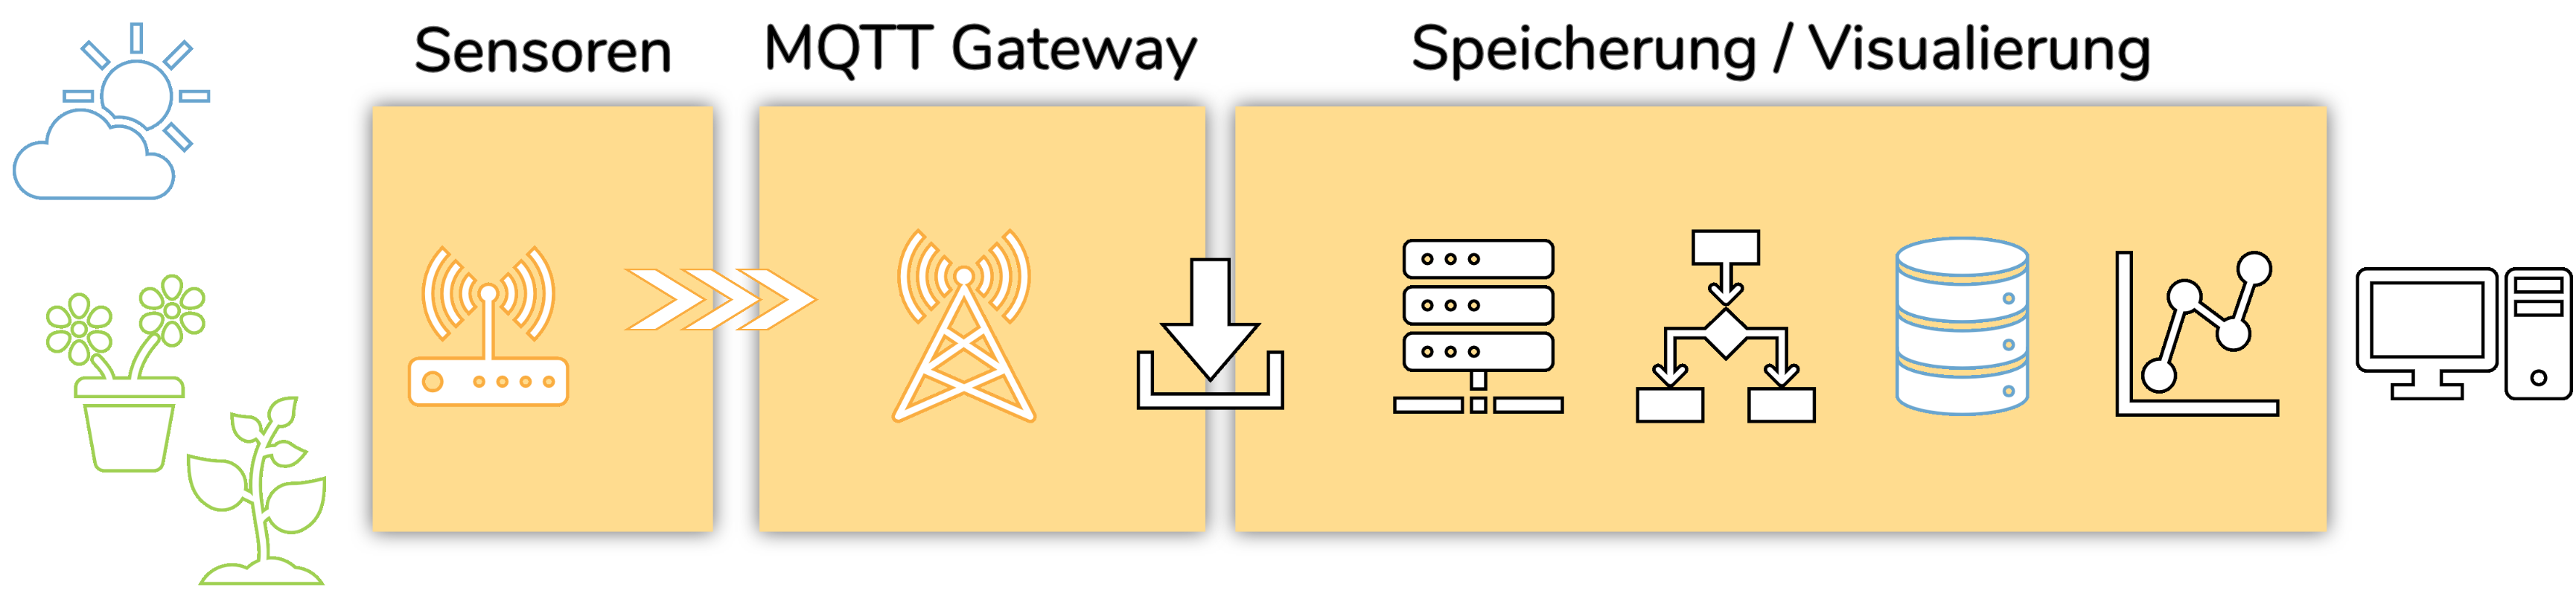
\includegraphics[width=18cm, left]{Bilder/Overview.png}
  \end{center}
    \caption{Systemaufbau}
\end{figure}

\chapter{Einleitung}
\section{Übersicht}
Die Komponenten wurden durch das Vorhandensein von Bibliotheken und Treibern sowie die leichte Beschaffung auch innerhalb der Schweiz bestimmt. Der Verzicht auf kommerzielle Systeme erlaubt eine grosse Flexibilität in der Kombination von Funktionalitäten.
\section{Hardware}

\chapter{Aufbau der Sensoren}
\section{Mikrokontroller}
Ein sehr beliebter Mikrokontroller ist der ESP32 von Espressif \cite{espressif} welcher durch grossen Funktionsumfang und einen recht geringen Preis überzeugen kann. Ein Vorteil ist ebenfalls die Möglichkeit der Programmierung durch die Arduino\cite{arduino} IDE welche frei verfügbar ist und die Entwicklung stark vereinfacht. Es existieren viele verschiedene Mikrocontroller welche den ESP32 Baustein verwenden, für dieses Projekt kam der Firebeetle \cite{firebeetle} von DF Robot zum Einsatz.  \footnote{https://www.bastelgarage.ch/firebeetle-esp32-iot-mikrocontroller-mit-wifi}

\begin{figure}[ht]
	\begin{minipage}[t]{0.5\linewidth}
		\centering
		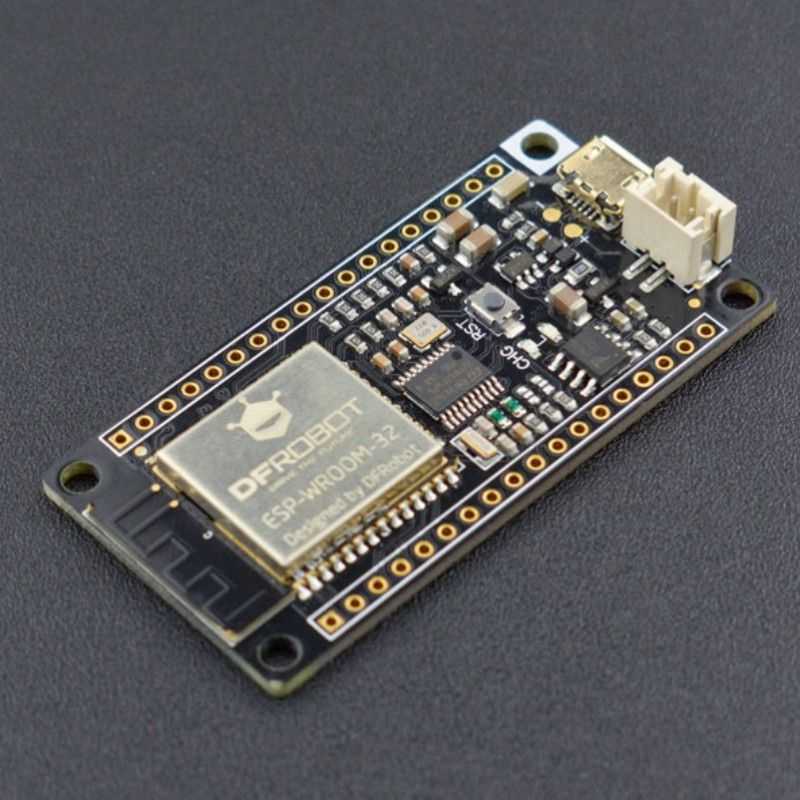
\includegraphics[ width=0.75\linewidth, valign=t]{Bilder/Firebeetle.jpg} 
		 \caption{Firebeetle mit dem ESP32 Mikrokontroller}
	\end{minipage}%
	\begin{minipage}[t]{0.5\linewidth}
	Der ESP32 besitzt sowohl WLAN als auch Bluetooth LE Schnittstellen. Diese wurden jedoch aus Gründen des Stromverbrauchs (WLAN) oder der Reichweite (Bluetooth LE) in diesem Projekt nicht verwendet.\break \break
	 Der Firebeetle\cite{firebeetle} Baustein hat sowohl die Möglichkeit einer Stromversorgung mit 5 Volt als auch mit 3.7 Volt, womit er direkt durch Lithium-Ionen Akkus betrieben werden kann.
	\end{minipage}
\end{figure}

 \section{Sensoren}
 Es existiert eine grosse Anzahl an verschiedenen Sensoren welche auch für Privatanwendern nutzbar sind. In diesem Projekt wurden Sensoren gewählt für welche frei verfügbare Bibliotheken in einer Version für den ESP32 vorhanden sind. Grundsätzlich wird bei den Sensoren unterschieden zwischen solchen die 
 \begin{itemize}
	 \item Digitale Werte liefern die direkt einer Einheit (Grad Celsius) oder Prozentangabe (Luftfeuchtigkeit) entsprechen
	  \item Analoge Messwerte welche auf eine Einheit umgerechnet werden müssen
\end{itemize}
 
 \subsection{Temperatur und Luftfeuchtigkeit}
 \subsubsection{DHT22}
 \begin{figure}[htp]
  \begin{center}
    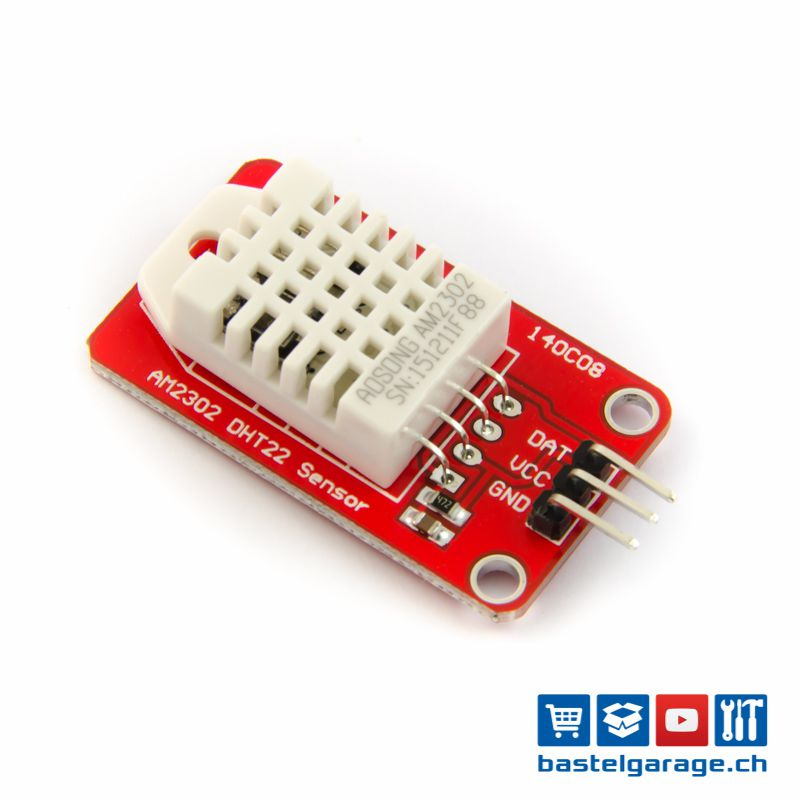
\includegraphics[width=5cm, left]{Bilder/DHT22.jpg}
  \end{center}
    \caption{Temperatur und Luftfeuchtigkeitsmesser DHT22}
  \label{fig:dht22}
\end{figure}
DHT22 im Onlineshop \footnote{https://www.bastelgarage.ch/dht22-temperatur-und-luftfeuchtigkeitssensor-steckbar}

\subsubsection{DHT11}
Als alternative zu dem oben genannten DHT22 gibt es eine billigere Variante mit dem Namen DHT11. \footnote{https://www.bastelgarage.ch/dht11-temperatur-und-luftfeuchtigkeitssensor?search=dht11}
\begin{figure}[ht]
	\begin{minipage}[t]{0.5\linewidth}
		\centering
		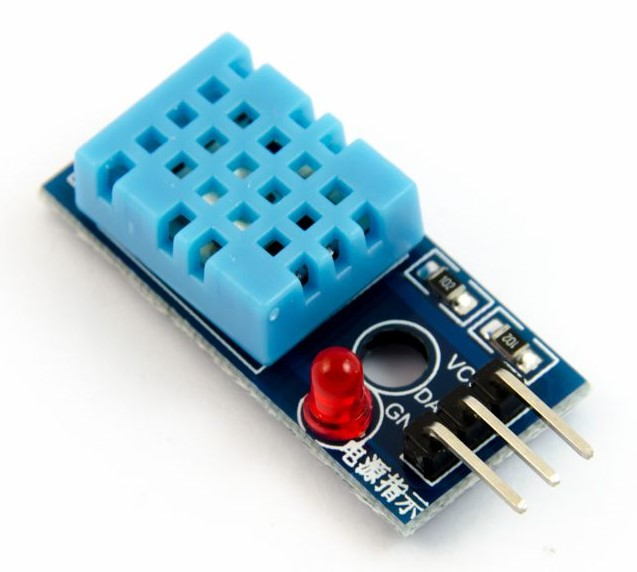
\includegraphics[ width=0.75\linewidth, valign=t]{Bilder/DHT11.jpg} 
		 \caption{DHT11 Luft- und Feuchtigkeitssensor}
	\end{minipage}%
	\begin{minipage}[t]{0.5\linewidth}
	Der DHT11 Sensor hat eine geringere Auflösung als der DHT22, ist ansonsten aber gleich verwendbar.
	\end{minipage}
\end{figure}

\subsection{Bodenfeuchtigkeit}

\begin{center}
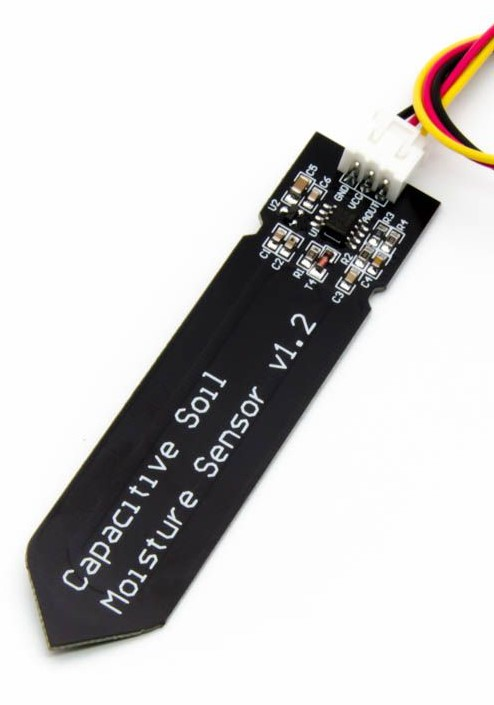
\includegraphics[width=5cm, left]{Bilder/Soil-2.jpg}%
\captionof{figure}{Kapazitiver Bodenfeuchtesensor V1.2}\label{labelname}%
\end{center}
Bodensensor im Onlineshop \footnote{https://www.bastelgarage.ch/bauteile/sensoren/kapazitiver-bodenfeuchtesensor-v1-2}

 \section{Funkverbindung}
\begin{center}
    \begin{minipage}[b]{0.45\textwidth}
        \centering
        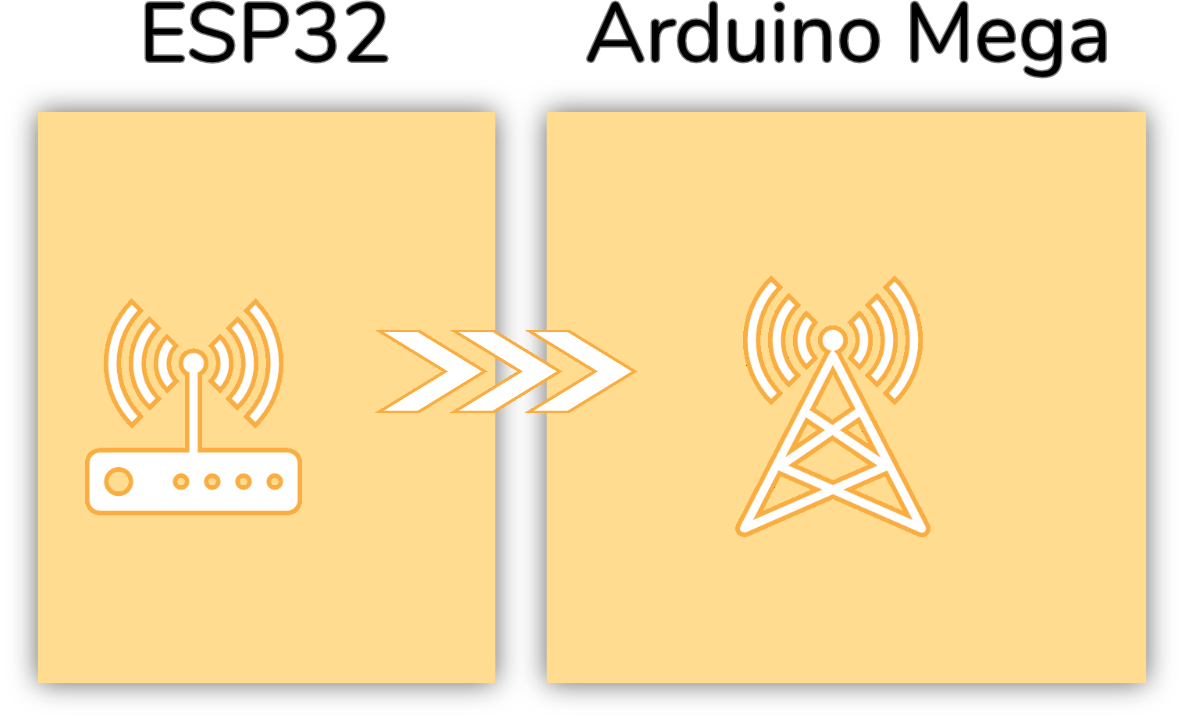
\includegraphics[width=7cm]{Bilder/ESP32-Arduino.png} % first figure itself
        \captionsetup{justification=centering}
        \captionof{figure}{Funkverbindung}
    \end{minipage}\hfill
    \begin{minipage}[b]{0.45\textwidth}
        \centering
        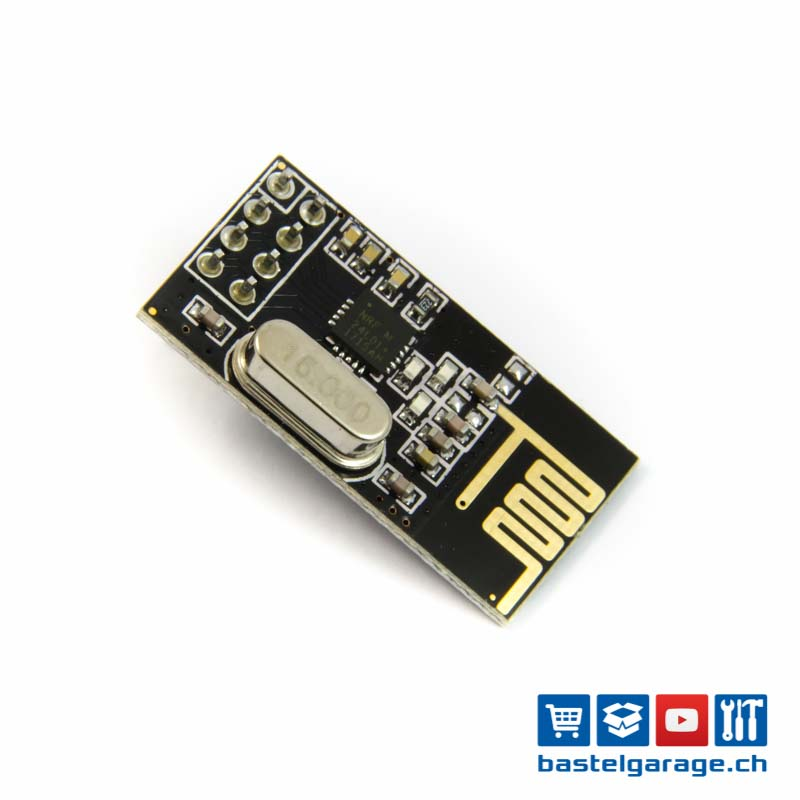
\includegraphics[width=5cm]{Bilder/NRF24.jpg} % second figure itself
        \captionsetup{justification=centering}
        \captionof{figure}{NRF24L01+ Funkmodul}
    \end{minipage}
\end{center}
NRF24L01+ \footnote{https://www.bastelgarage.ch/bauteile/funk-wireless-lora/nrf24l01-wireless-funk-modul-2-4ghz}
 \begin{listing}[h]
 \begin{minted}[frame=single,
               framesep=3mm,
               linenos=true,
               xleftmargin=10pt,
               tabsize=4,
               fontsize=\small]{js}
 3A51266ABD432C1FB797DEDEE215FD16E42BAB627F104BCB6F4169EDE4544582:4;25.1;71.1;10.2
 \end{minted}
  \caption{Format des Datensatz über Funk}
 \end{listing}

 \section{Software}

%
\chapter{IoT Gateway}
\section{Übersicht}
\section{Hardware}
\section{Funkverbindung}
\subsection{Zugriffsschutz}
Jede empfangene Nachricht wird durch die Valdierung des HMAC (\Gls{HMAC}) sowohl auf einen berechtigten Absender, als auch auf unverfälschte Daten überprüft.
\section{Software}
\chapter{Speicherung und Visualisierung}
\section{Übersicht}
\begin{center}
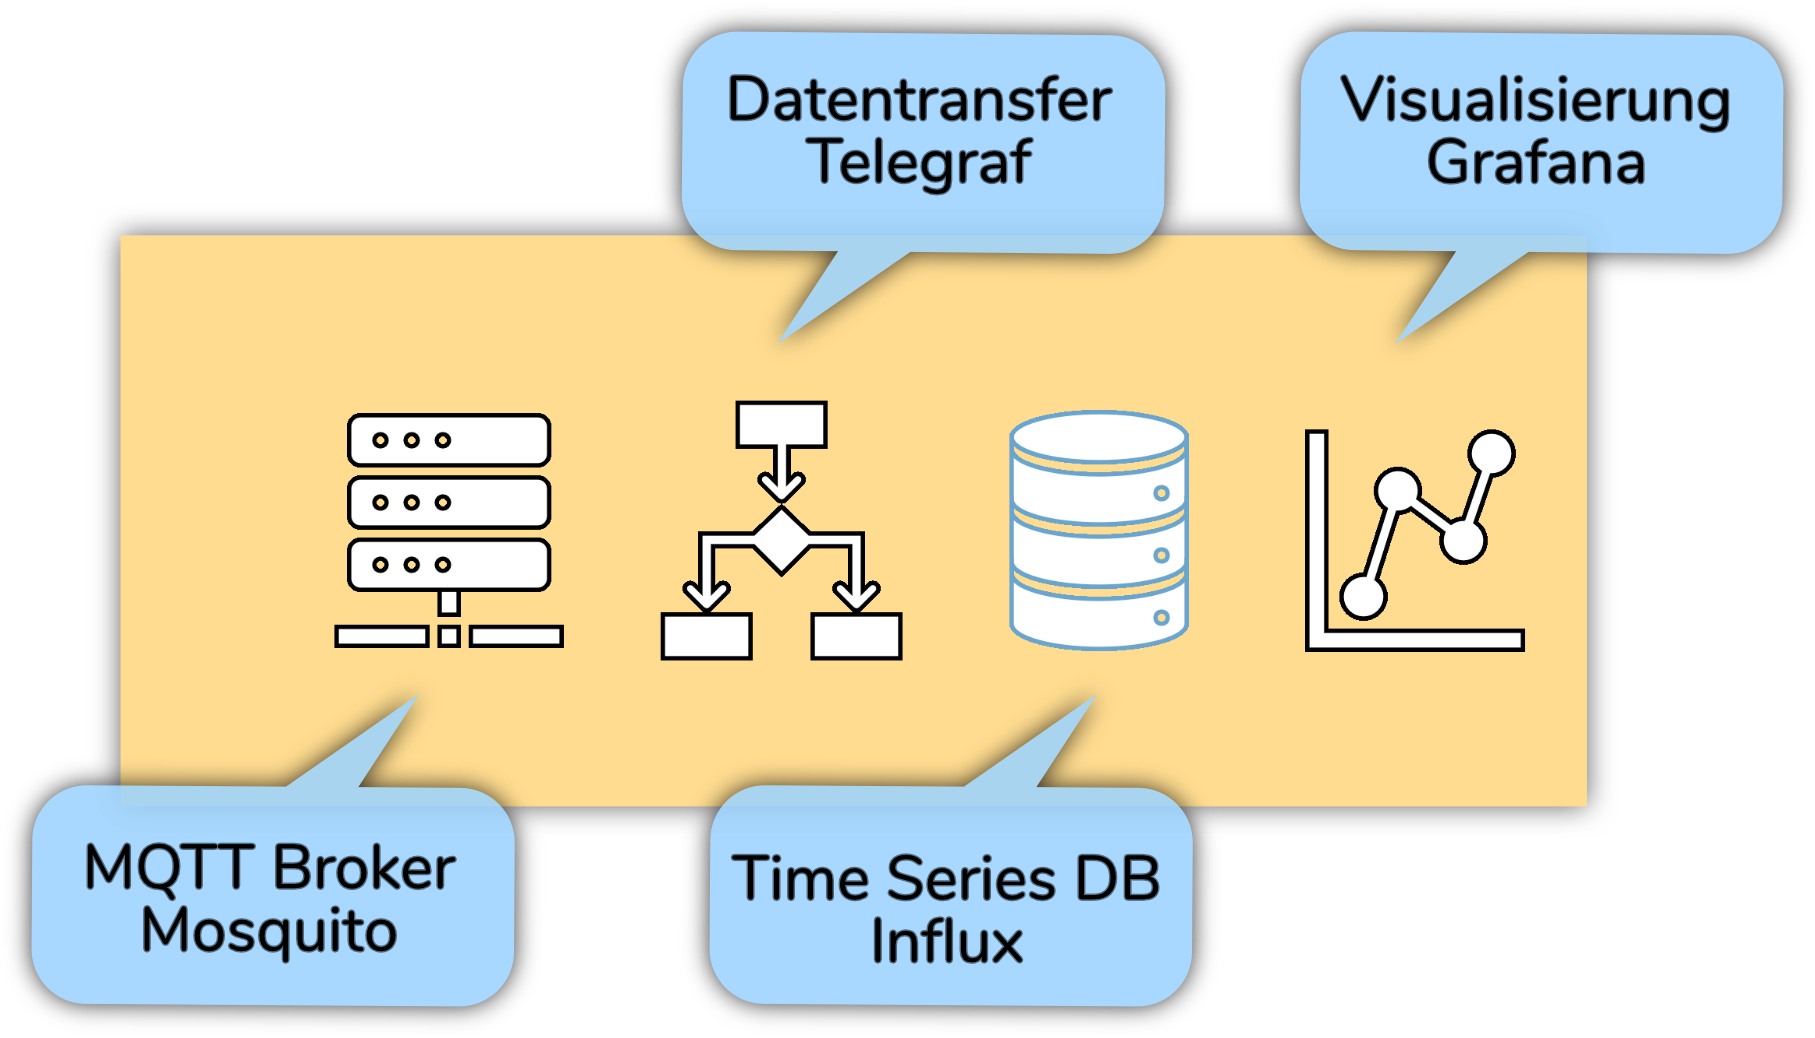
\includegraphics[width=17cm, left]{Bilder/Raspberry-Software.png}%
\captionof{figure}{Verwendete Software}\label{labelname}%
\end{center}
\section{Hardware}
\section{Visualisierung}
\begin{listing}
\begin{minted}[frame=single,
               framesep=3mm,
               linenos=true,
               xleftmargin=21pt,
               tabsize=4]{js}
{     
    "firstName": "John"
    "lastName" : "Smith",
    "age" : 25
}
\end{minted}
\caption{JSON example} 
\label{json-example}
\end{listing}

% List of Figures
\listoffigures
% List of Tables
\listoftables
% Glossary
\printglossary
% Bibliography

\renewcommand\bibname{Linkverzeichnis}
\begin{thebibliography}{99}
   \bibitem{whyHmac} What is HMAC Authentication and why is it useful?\break \url{https://www.wolfe.id.au/2012/10/20/what-is-hmac-authentication-and-why-is-it-useful/}
    \bibitem{esp32-hmac} ESP32 Arduino: Applying the HMAC SHA-256 mechanism\break \url{https://techtutorialsx.com/2018/01/25/esp32-arduino-applying-the-hmac-sha-256-mechanism/}
    \bibitem{hmacOnline} Online HMAC Code Generator\break \url{https://www.freeformatter.com/hmac-generator.html#ad-output}
    \bibitem{nrf24} NRF24L01+ Funkmodul Treiber für Arduino und ESP32\break \url{http://tmrh20.github.io/RF24/index.html}
    \bibitem{espressif} Herstellerseite Espressif für den ESP32\break \url{https://www.espressif.com/en/products/hardware/esp32/overview}
    \bibitem{arduino} Arduino Herstellerseite mit der gleichnamigen IDE und vielen Bibliotheken und Tutorials\break \url{https://www.arduino.cc/}
    \bibitem{firebeetle} Herstellerseite des Firebeetle Mikrokontrollers\break \url{https://www.dfrobot.com/product-1590.html}
  \end{thebibliography}
%Index
\addcontentsline{toc}{chapter}{Index}
%\printindex
% Appendices
\end{document}
